\chapter{x86 Explained}
\label{chapter:usecase}

This Chapter takes the x86 hardware architecture as an example to illustrate the
challenge related to hardware-based security enforcement.
%
Because of its predominant position, the x86 architectures has been particularly
studied over the past decade.
%
As a consequence, there are a lot of resources on the subject.
%
That being said, other mainstream architectures (\emph{e.g.} ARM) work on
similar basis and suffer similar issues.

At the time of writing this thesis\,\footnote{Spring 2018.}, the \emph{Intel 64
  and IA-32 Architectures Software Developer’s Manual} is 4842 pages long.
%
The output of \texttt{lshw -short} on one regular computer lists about 30
hardware components in addition to the main CPU.
%
Each of them come with its own documentations, often in the form of large
datasheets.
%
This means the information about how the computing platform works are scattered
throughout many sources.
%
This situation inevitably complicates the work of low-level software developers.
%
From a security perspective, they need to have a comprehensive view of how the
computing platform works as a whole.
%
This problematic also exists for hardware designers.
%
When they want to add a new feature, or a new component, they have to be certain
they will not break existing properties of the architecture by doing so.

This Chapter proceeds as follows:
%
we describe in more detail how a typical x86 computing platform work, that is
which king of hardware components are involved, which kind of software stack
they execute, and how they interact with each others
(Section\,\ref{sec:usecase:architecture});
%
we focus on the key role played by the firmware in the platform functioning and
security (Section\,\ref{sec:usecase:firmware});
%
we detail several HSE mechanisms implemented by the firmware, including how they
have been compromised (Section\,\ref{sec:usecase:hse}).

\section{x86 Computing Platform Explained}
\label{sec:usecase:architecture}

Describing a computing platform in depth is challenging, because it is made of
many interdependent components of various nature.
%
As a consequence, we start our explanation from the typical abstraction layers
which form a computing platform, then deconstruct them in order to detail how
they are concretely implemented.

\subsection{Typical Software Stack}

Figure\,\ref{fig:usecase:computing-platform-1} pictures the traditional
abstraction layers of a computing platform.

\begin{description}
\item [Hardware] The physical components that together form the computer, whose
  purpose is to run software components users can interact with.
%
\item [Firmware] In the context of this thesis, we call firmware a software
  component shipped with a particular hardware component by its vendor to ensure
  its correct functioning.
%
\item [Operating System] A system software whose main purpose is to manage
  hardware resources among several applications.
%
\item [End-user application] One could say the lower layers only exist to allow
  applications to focus on business logic.
\end{description}

Each layer leverages the interface of its predecessor to expose a higher-level,
more constrained set of functionalities for its successors.
%
Thus, software developers who write end-user application do not need to handle
the complexity of x86, thanks to the principle of separation of concern: while
the underlying operating system (and the firmware) handles the hardware specific
tasks, they can focus on application logic.
%
These interfaces are often standardize to some extend, which allows
interoperability.
%
This is useful because the market is characterized by a large diversity of
products.
%
%For instance, to abstract away the specificity of each vendors
%of existing products: UEFI (firmware), POSIX (operating system), etc.

Each layer is more privileged than its successors:
%
the hardware architecture executes the software stack;
%
the firmware has the mean to interrupt the execution of the other software
components;
%
the operating system loads in memory and manages the applications the user can
interact with.

\begin{figure}
  \centering
  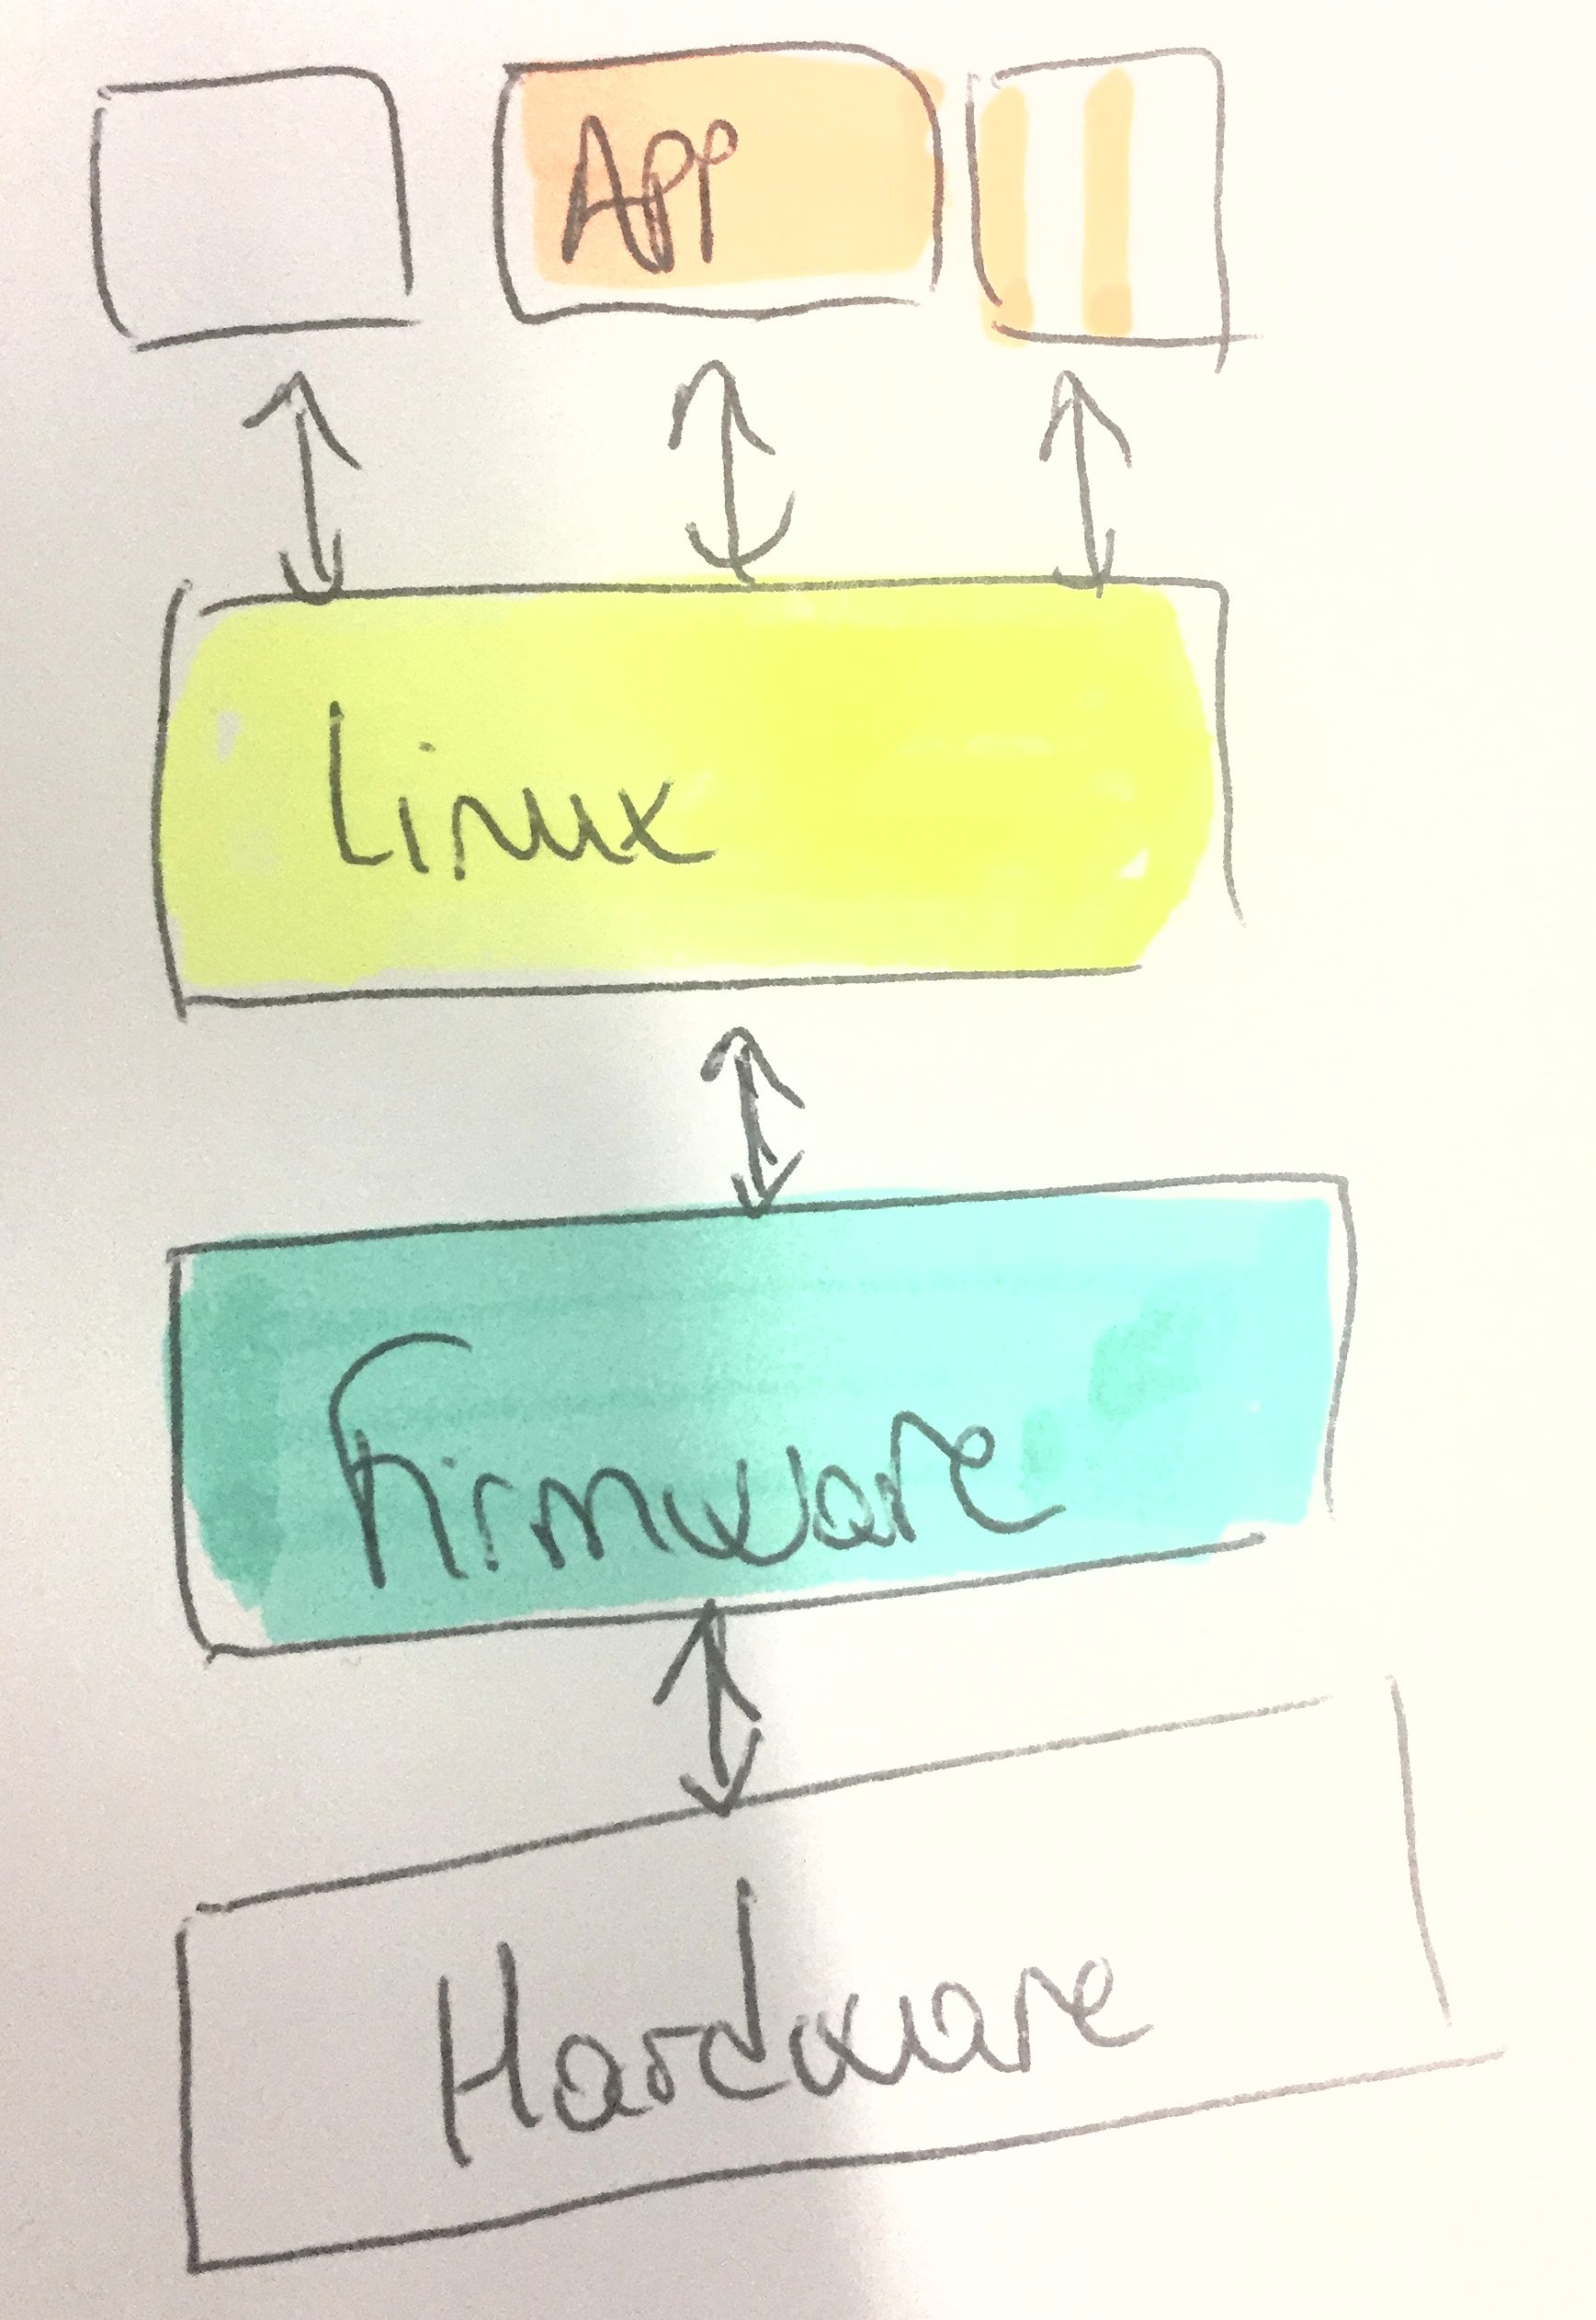
\includegraphics[width=0.3\textwidth]{Figures/computing-platform-1.jpg}
  \caption{Abstraction Layers of a Typical x86 Computing Platform}
  \label{fig:usecase:computing-platform-1}
\end{figure}

\subsection{Concurrent Software Stacks}

If the abstractions pictured in Figure\,\ref{fig:usecase:computing-platform-1}
are often well understood by software developers, it is less acknowledge that
there are many software stacks inside one computer.
%
Figure\,\ref{fig:usecase:computing-platform-2} gives a glimpse of software stack
diversity inside a computer.

\begin{figure}
  \centering
  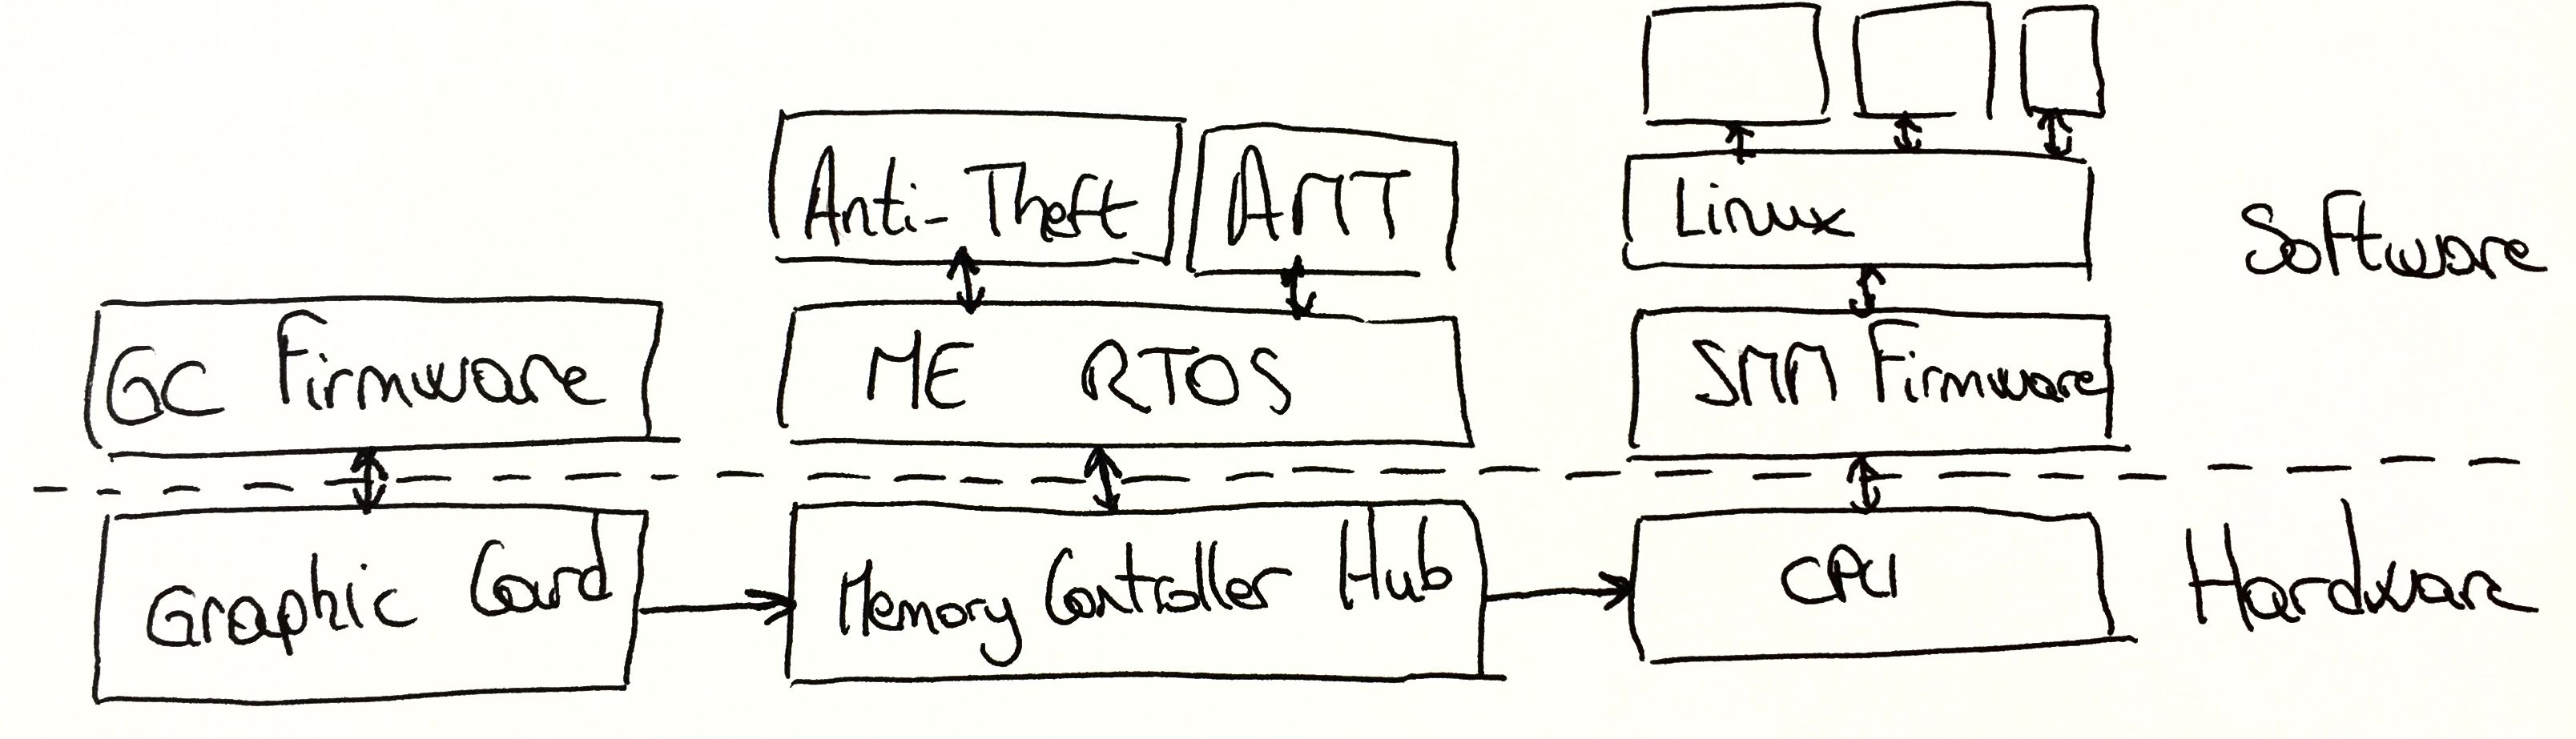
\includegraphics[width=0.8\textwidth]{Figures/intro-computing-platform.jpg}
  \caption{Multiple Software Stacks in x86 Hardware Architecture}
  \label{fig:usecase:computing-platform-2}
\end{figure}

\subsection{Hardware-Software}

Figure xx
%
This makes \emph{isolation} a key security property.
%
In the context of this thesis, we say one component $A$ is said isolated from a
second component $B$ when $B$ cannot tamper with $A$'s functioning otherwise
than through its interface.
%
Thus, an operating system should be isolated from end users applications, to
prevent the latter to grant themselves abusive rights.
%
The opposite is not necessarily true, and it is even a common practice for
operating system to tamper with applications code (\emph{e.g.} address space
layout randomization, dynamic libraries).

\begin{figure}
  \centering
  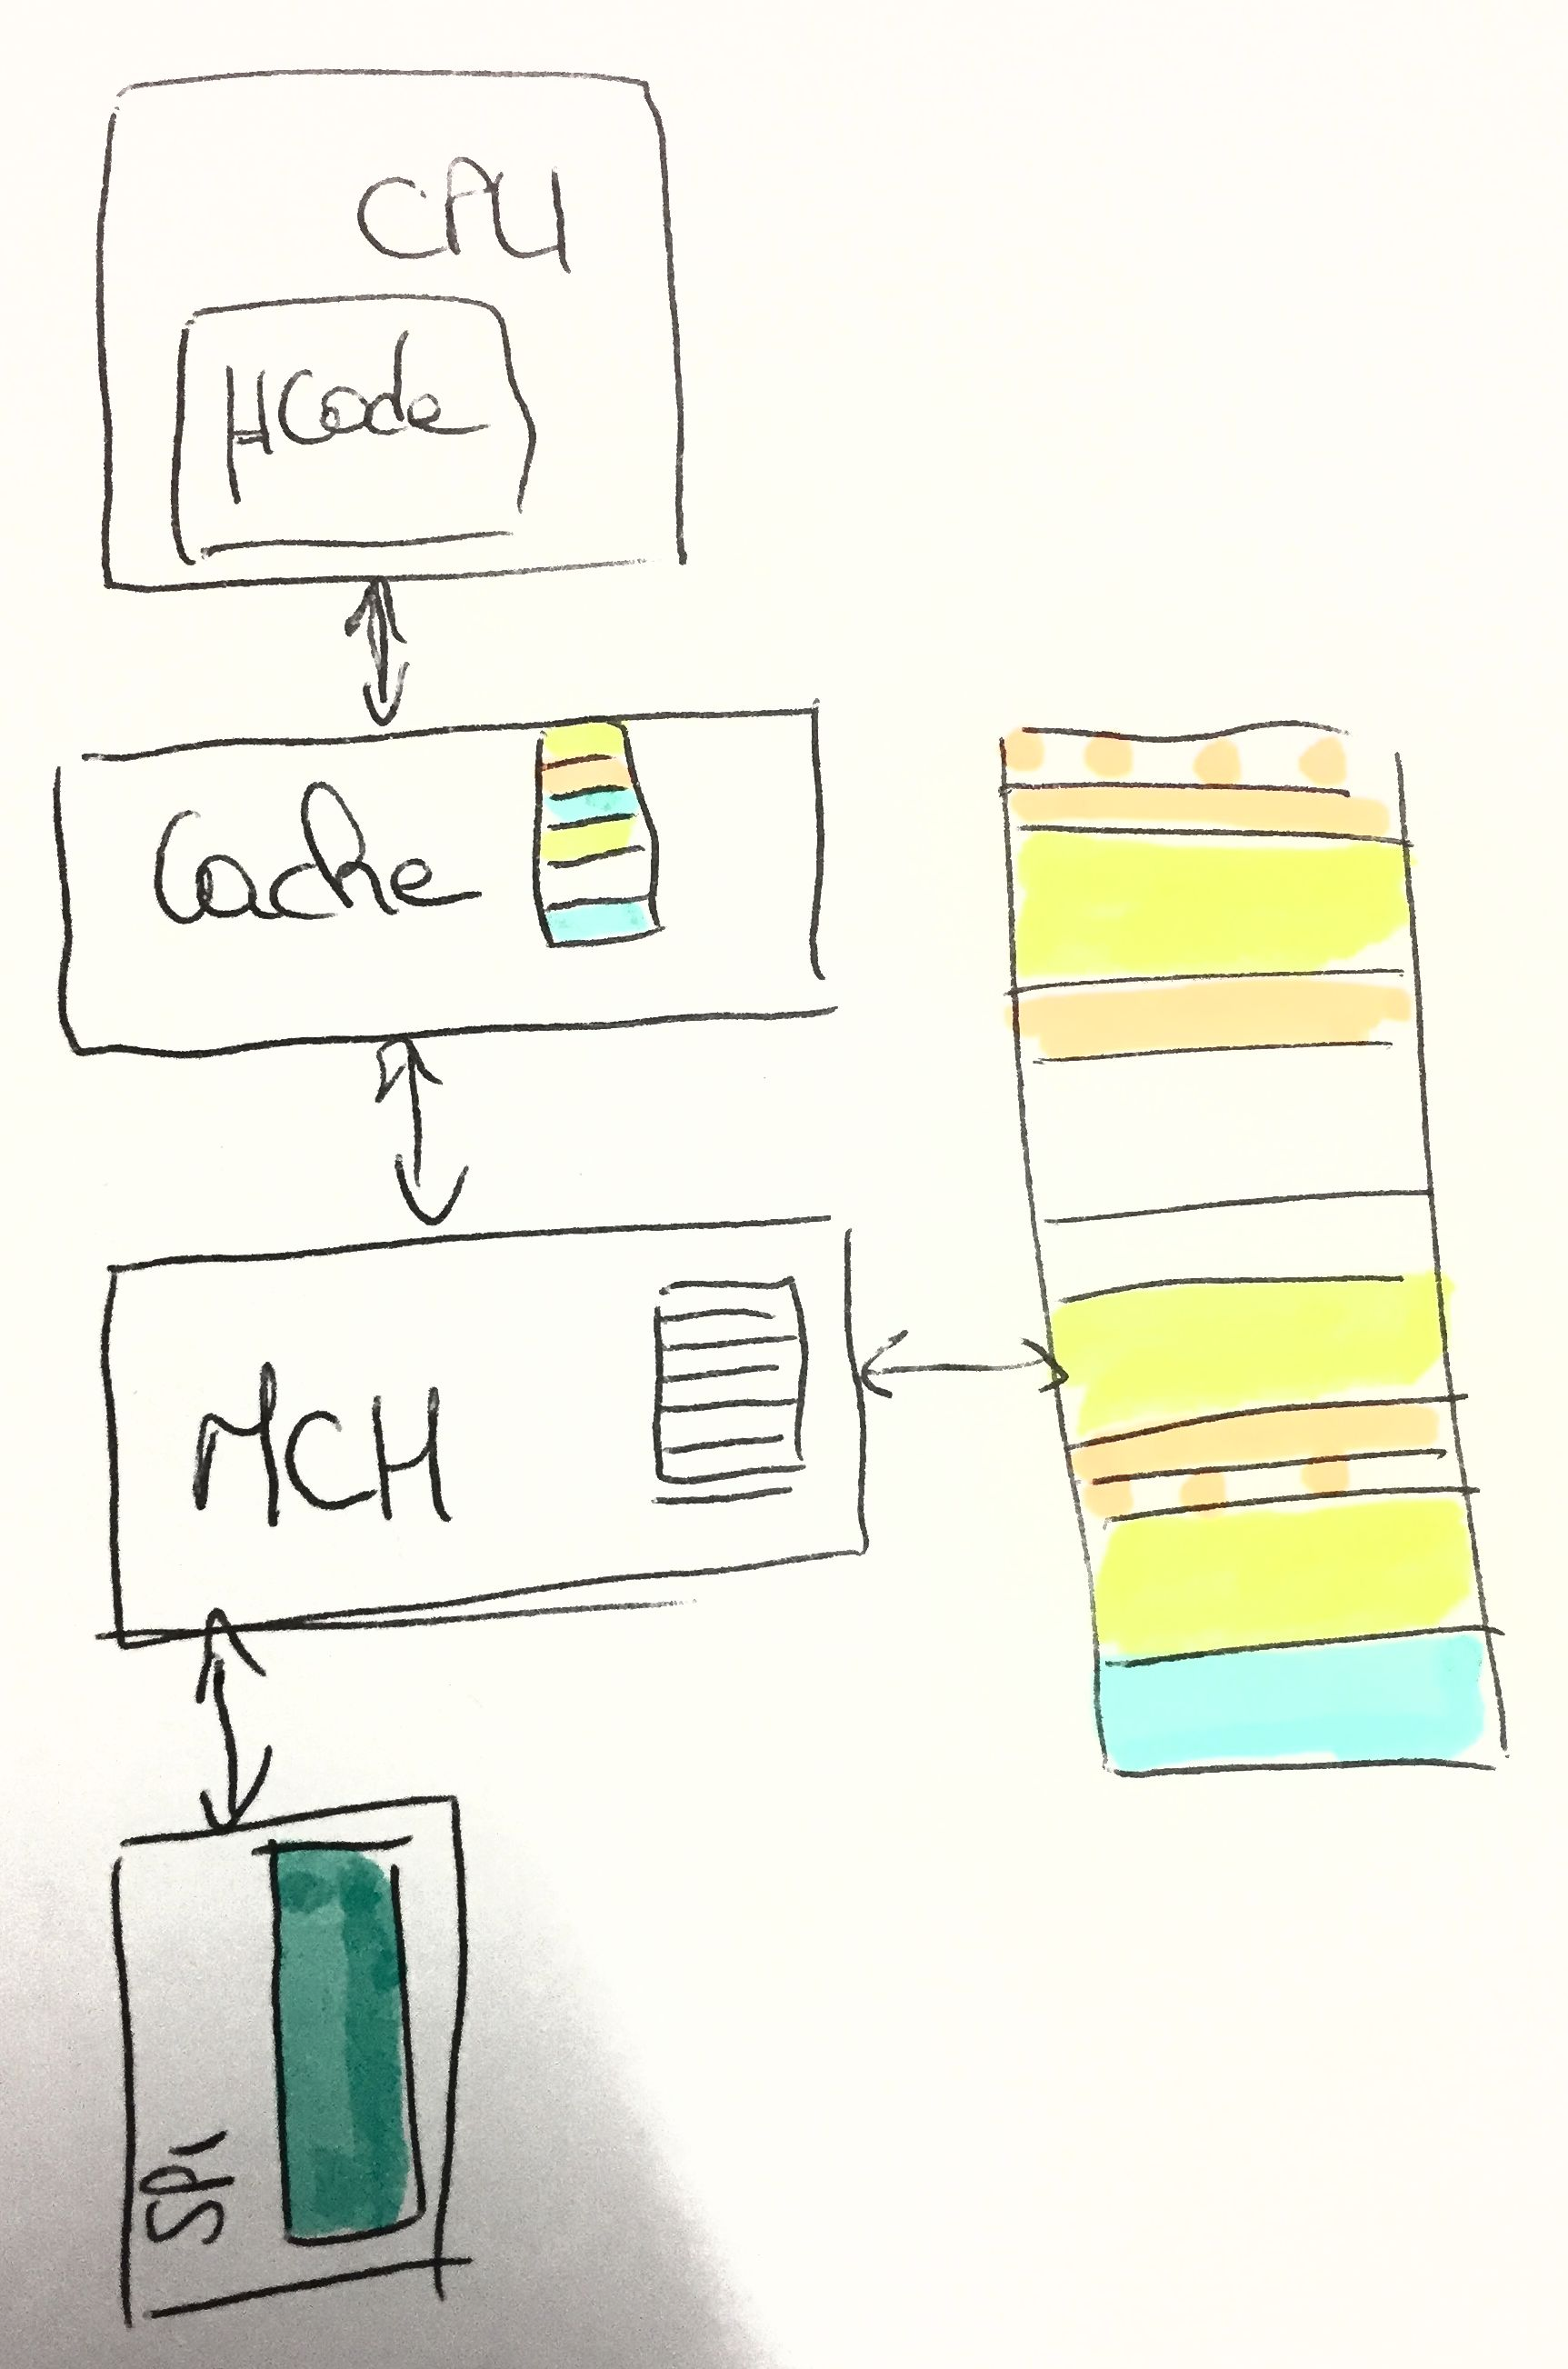
\includegraphics[width=0.3\textwidth]{Figures/computing-platform-3.jpg}
  \caption{Abstraction Layers of a Typical x86 Computing Platform}
  \label{fig:usecase:computing-platform-3}
\end{figure}

\thomasrk[inline]{What we want to write in a glimpse:}

\begin{description}
\item [Figure 2] Le HW n’est pas un bloc uniforme, et d’autres software stacks
  sont exécutés en même temps (citer Navy/attaque de YAP, pour souligner que
  c’est important)
\item [Figure 3] Le SW n'existe pas a proprement parlé, il est éclaté entre
  plusieurs localisations; être en mesure de contrôler ce que l’autre exécute,
  c’est gagner la partie
\end{description}


\section{Firmware}
\label{sec:usecase:firmware}

\section{Firmware HSE}
\label{sec:usecase:hse}

\section{Conclusion}
\label{sec:usecase:conclusion}
